%
% template.tex -- slide template
%
% (c) 2021 Prof Dr Andreas Müller, OST Ostschweizer Fachhochschule
%
\bgroup
\def\a{2}
\def\b{0.8}
\def\c{1}
\def\d{0.6}
\def\vnull{
	\coordinate (A) at ({0*\a},0);
	\coordinate (B) at ({1*\a},0);
	\coordinate (C) at ({2*\a},0);
	\coordinate (D) at ({0.5*\a},{-\b});
	\coordinate (E) at ({1.5*\a},{-\b});
	\draw (A) -- (B);
	\draw (A) -- (D);
	\draw (B) -- (C);
	\draw (B) -- (D);
	\draw (B) -- (E);
	\draw (C) -- (E);
	\draw (D) -- (E);
	\node at (-2.8,{-0.5*\b}) [right] {$\lambda=0.0000$};
	\fill[color=red!100] (A) circle[radius=0.25];
	\draw (A) circle[radius=0.25];
	\fill[color=red!100] (B) circle[radius=0.25];
	\draw (B) circle[radius=0.25];
	\fill[color=red!100] (C) circle[radius=0.25];
	\draw (C) circle[radius=0.25];
	\fill[color=red!100] (D) circle[radius=0.25];
	\draw (D) circle[radius=0.25];
	\fill[color=red!100] (E) circle[radius=0.25];
	\draw (E) circle[radius=0.25];
}
\def\fnull{
	\draw[color=red,line width=1.4pt]
		({-2.0000*\c},{0.4472*\d}) --
		({-1.0000*\c},{0.4472*\d}) --
		({0.0000*\c},{0.4472*\d}) --
		({1.0000*\c},{0.4472*\d}) --
		({2.0000*\c},{0.4472*\d});
	\draw[->] ({-2.1*\c},0) -- ({2.1*\c},0);
	\draw[->] (0,{-1.1*\d}) -- (0,{1.1*\d});
	\fill ({-2*\c},0) circle[radius=0.05];
	\fill ({-1*\c},0) circle[radius=0.05];
	\fill ({0*\c},0) circle[radius=0.05];
	\fill ({1*\c},0) circle[radius=0.05];
	\fill ({2*\c},0) circle[radius=0.05];
}
\def\vone{
	\coordinate (A) at ({0*\a},0);
	\coordinate (B) at ({1*\a},0);
	\coordinate (C) at ({2*\a},0);
	\coordinate (D) at ({0.5*\a},{-\b});
	\coordinate (E) at ({1.5*\a},{-\b});
	\draw (A) -- (B);
	\draw (A) -- (D);
	\draw (B) -- (C);
	\draw (B) -- (D);
	\draw (B) -- (E);
	\draw (C) -- (E);
	\draw (D) -- (E);
	\node at (-2.8,{-0.5*\b}) [right] {$\lambda=0.1586$};
	\fill[color=blue!100] (A) circle[radius=0.25];
	\draw (A) circle[radius=0.25];
	\fill[color=blue!00] (B) circle[radius=0.25];
	\draw (B) circle[radius=0.25];
	\fill[color=red!100] (C) circle[radius=0.25];
	\draw (C) circle[radius=0.25];
	\fill[color=blue!41] (D) circle[radius=0.25];
	\draw (D) circle[radius=0.25];
	\fill[color=red!41] (E) circle[radius=0.25];
	\draw (E) circle[radius=0.25];
}
\def\fone{
	\draw[color=red,line width=1.4pt]
		({-2.0000*\c},{-0.6533*\d}) --
		({-1.0000*\c},{-0.2706*\d}) --
		({0.0000*\c},{-0.0000*\d}) --
		({1.0000*\c},{0.2706*\d}) --
		({2.0000*\c},{0.6533*\d});
	\draw[->] ({-2.1*\c},0) -- ({2.1*\c},0);
	\draw[->] (0,{-1.1*\d}) -- (0,{1.1*\d});
	\fill ({-2*\c},0) circle[radius=0.05];
	\fill ({-1*\c},0) circle[radius=0.05];
	\fill ({0*\c},0) circle[radius=0.05];
	\fill ({1*\c},0) circle[radius=0.05];
	\fill ({2*\c},0) circle[radius=0.05];
}
\def\vtwo{
	\coordinate (A) at ({0*\a},0);
	\coordinate (B) at ({1*\a},0);
	\coordinate (C) at ({2*\a},0);
	\coordinate (D) at ({0.5*\a},{-\b});
	\coordinate (E) at ({1.5*\a},{-\b});
	\draw (A) -- (B);
	\draw (A) -- (D);
	\draw (B) -- (C);
	\draw (B) -- (D);
	\draw (B) -- (E);
	\draw (C) -- (E);
	\draw (D) -- (E);
	\node at (-2.8,{-0.5*\b}) [right] {$\lambda=0.3000$};
	\fill[color=red!100] (A) circle[radius=0.25];
	\draw (A) circle[radius=0.25];
	\fill[color=blue!00] (B) circle[radius=0.25];
	\draw (B) circle[radius=0.25];
	\fill[color=red!100] (C) circle[radius=0.25];
	\draw (C) circle[radius=0.25];
	\fill[color=blue!100] (D) circle[radius=0.25];
	\draw (D) circle[radius=0.25];
	\fill[color=blue!100] (E) circle[radius=0.25];
	\draw (E) circle[radius=0.25];
}
\def\ftwo{
	\draw[color=red,line width=1.4pt]
		({-2.0000*\c},{0.5000*\d}) --
		({-1.0000*\c},{-0.5000*\d}) --
		({0.0000*\c},{-0.0000*\d}) --
		({1.0000*\c},{-0.5000*\d}) --
		({2.0000*\c},{0.5000*\d});
	\draw[->] ({-2.1*\c},0) -- ({2.1*\c},0);
	\draw[->] (0,{-1.1*\d}) -- (0,{1.1*\d});
	\fill ({-2*\c},0) circle[radius=0.05];
	\fill ({-1*\c},0) circle[radius=0.05];
	\fill ({0*\c},0) circle[radius=0.05];
	\fill ({1*\c},0) circle[radius=0.05];
	\fill ({2*\c},0) circle[radius=0.05];
}
\def\vthree{
	\coordinate (A) at ({0*\a},0);
	\coordinate (B) at ({1*\a},0);
	\coordinate (C) at ({2*\a},0);
	\coordinate (D) at ({0.5*\a},{-\b});
	\coordinate (E) at ({1.5*\a},{-\b});
	\draw (A) -- (B);
	\draw (A) -- (D);
	\draw (B) -- (C);
	\draw (B) -- (D);
	\draw (B) -- (E);
	\draw (C) -- (E);
	\draw (D) -- (E);
	\node at (-2.8,{-0.5*\b}) [right] {$\lambda=0.4414$};
	\fill[color=red!41] (A) circle[radius=0.25];
	\draw (A) circle[radius=0.25];
	\fill[color=red!00] (B) circle[radius=0.25];
	\draw (B) circle[radius=0.25];
	\fill[color=blue!41] (C) circle[radius=0.25];
	\draw (C) circle[radius=0.25];
	\fill[color=blue!100] (D) circle[radius=0.25];
	\draw (D) circle[radius=0.25];
	\fill[color=red!100] (E) circle[radius=0.25];
	\draw (E) circle[radius=0.25];
}
\def\fthree{
	\draw[color=red,line width=1.4pt]
		({-2.0000*\c},{0.2706*\d}) --
		({-1.0000*\c},{-0.6533*\d}) --
		({0.0000*\c},{0.0000*\d}) --
		({1.0000*\c},{0.6533*\d}) --
		({2.0000*\c},{-0.2706*\d});
	\draw[->] ({-2.1*\c},0) -- ({2.1*\c},0);
	\draw[->] (0,{-1.1*\d}) -- (0,{1.1*\d});
	\fill ({-2*\c},0) circle[radius=0.05];
	\fill ({-1*\c},0) circle[radius=0.05];
	\fill ({0*\c},0) circle[radius=0.05];
	\fill ({1*\c},0) circle[radius=0.05];
	\fill ({2*\c},0) circle[radius=0.05];
}
\def\vfour{
	\coordinate (A) at ({0*\a},0);
	\coordinate (B) at ({1*\a},0);
	\coordinate (C) at ({2*\a},0);
	\coordinate (D) at ({0.5*\a},{-\b});
	\coordinate (E) at ({1.5*\a},{-\b});
	\draw (A) -- (B);
	\draw (A) -- (D);
	\draw (B) -- (C);
	\draw (B) -- (D);
	\draw (B) -- (E);
	\draw (C) -- (E);
	\draw (D) -- (E);
	\node at (-2.8,{-0.5*\b}) [right] {$\lambda=0.5000$};
	\fill[color=red!25] (A) circle[radius=0.25];
	\draw (A) circle[radius=0.25];
	\fill[color=blue!100] (B) circle[radius=0.25];
	\draw (B) circle[radius=0.25];
	\fill[color=red!25] (C) circle[radius=0.25];
	\draw (C) circle[radius=0.25];
	\fill[color=red!25] (D) circle[radius=0.25];
	\draw (D) circle[radius=0.25];
	\fill[color=red!25] (E) circle[radius=0.25];
	\draw (E) circle[radius=0.25];
}
\def\ffour{
	\draw[color=red,line width=1.4pt]
		({-2.0000*\c},{0.2236*\d}) --
		({-1.0000*\c},{0.2236*\d}) --
		({0.0000*\c},{-0.8944*\d}) --
		({1.0000*\c},{0.2236*\d}) --
		({2.0000*\c},{0.2236*\d});
	\draw[->] ({-2.1*\c},0) -- ({2.1*\c},0);
	\draw[->] (0,{-1.1*\d}) -- (0,{1.1*\d});
	\fill ({-2*\c},0) circle[radius=0.05];
	\fill ({-1*\c},0) circle[radius=0.05];
	\fill ({0*\c},0) circle[radius=0.05];
	\fill ({1*\c},0) circle[radius=0.05];
	\fill ({2*\c},0) circle[radius=0.05];
}

\begin{frame}[t]
\setlength{\abovedisplayskip}{5pt}
\setlength{\belowdisplayskip}{5pt}
\frametitle{Laplace-Basis}
\begin{center}
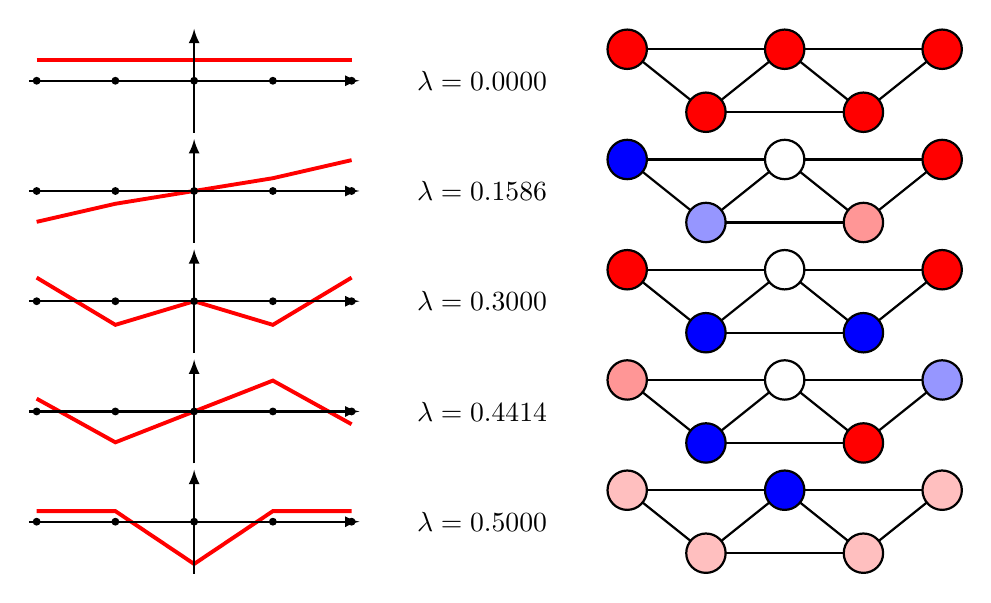
\begin{tikzpicture}[>=latex,thick]

\begin{scope}[yshift=-0.4cm,xshift=-5.5cm]]
\fnull
\end{scope}

\begin{scope}[yshift=-1.8cm,xshift=-5.5cm]]
\fone
\end{scope}

\begin{scope}[yshift=-3.2cm,xshift=-5.5cm]]
\ftwo
\end{scope}

\begin{scope}[yshift=-4.6cm,xshift=-5.5cm]]
\fthree
\end{scope}

\begin{scope}[yshift=-6.0cm,xshift=-5.5cm]]
\ffour
\end{scope}

\begin{scope}[yshift=0cm]
\vnull
\end{scope}

\begin{scope}[yshift=-1.4cm]
\vone
\end{scope}

\begin{scope}[yshift=-2.8cm]
\vtwo
\end{scope}

\begin{scope}[yshift=-4.2cm]
\vthree
\end{scope}

\begin{scope}[yshift=-5.6cm]
\vfour
\end{scope}

\end{tikzpicture}
\end{center}
\end{frame}
\egroup
